\section[Dynamic Monitoring Component Design]{A Dynamic Monitoring Component of a Data Flow testing tool}\label{tool}

In this project I designed, implemented and tested a component for a data flow software testing tool for Java programs called \datec. 

\paragraph{}
Figure~\ref{implem} summarizes the behavior of the data flow testing tool: the Static Analysis component, that was already implemented, statically analyzes source code to identify the data flow test requirements, and saves them in a MySql database. The Dynamic Monitor component I implemented then reads and interprets the data from the database, and during the execution of a test suite of the analyzed project, checks which data flow test requirements have been covered, producing a final report at the end of the execution. 

This section describes the challenges, design and implementation choices of the Dynamic Monitor component. 

 \begin{figure}[h]
   \begin{center}
   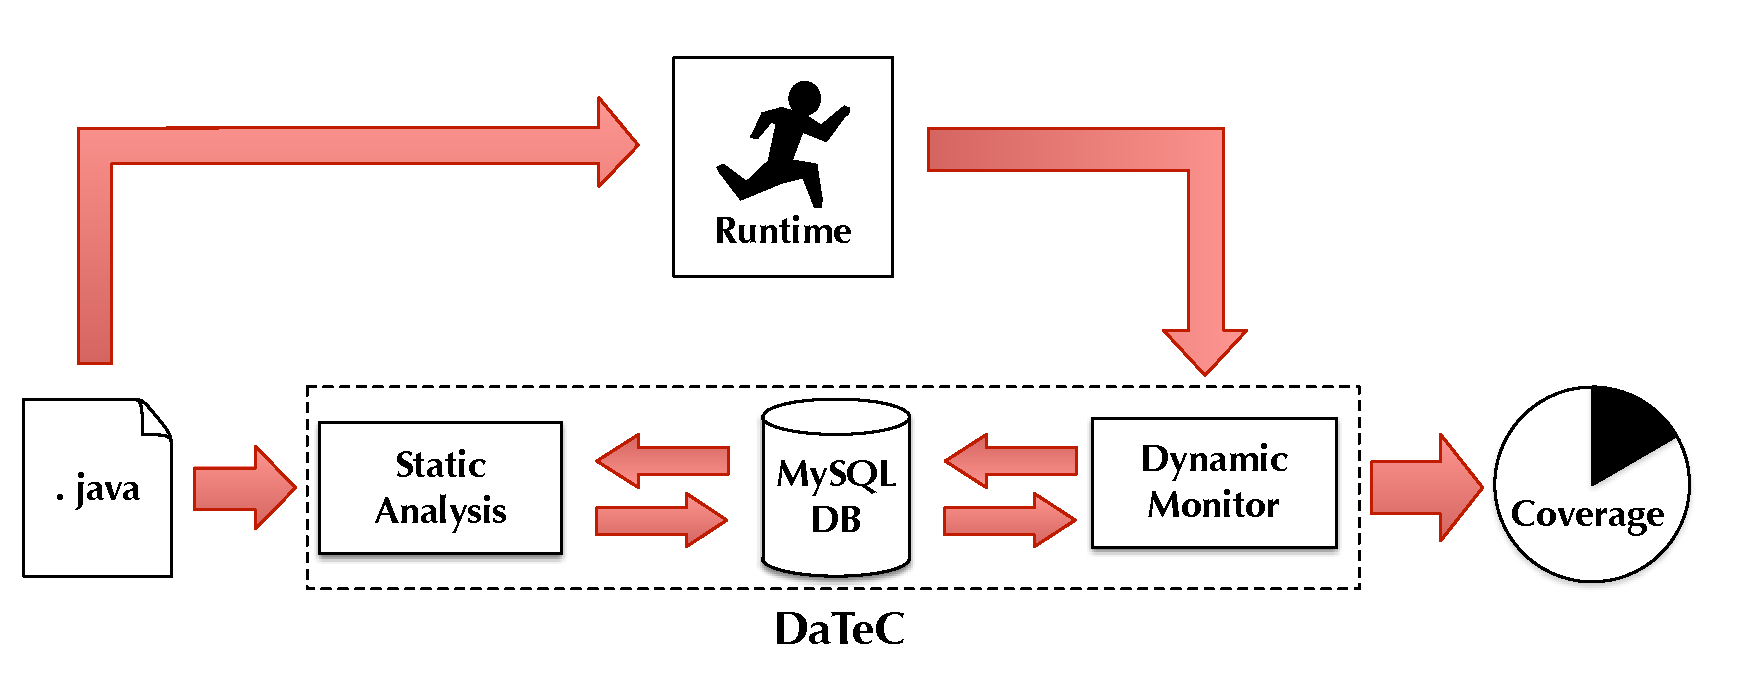
\includegraphics[width=\textwidth]{./Images/implementation.pdf}
   \caption{Implementation of the data flow testing tool}
  \label{implem}
  \end{center}
 \end{figure}

\subsection{Overview} 
The Dynamic Monitor performs three main steps to compute the data flow coverage of a given test suite:  
\begin{enumerate}
  \item Reads and interprets the data flow test objectives identified by the static analysis from the database;
  \item Instruments the program under analysis and dynamically monitor the execution to identify covered definition-use pairs;
  \item Updates the coverage information of the data flow test requirements identified statically and return a final report of the execution.
\end{enumerate}

\paragraph{}
The dynamic monitor exploits modular design (Figure \ref{modules}). 
\textit{StaticDB Interface} carries out the import and manipulation of the static analysis results. \textit{Active Fields Manager} instruments the program and monitors covered definition-use pairs. Finally, \textit{Report Manager} handles the presentation of the results in a format chosen by the user.
The role of each module will be discussed in relation to the function it carries out in the next sections.

 \begin{figure}[H]
   \begin{center}
   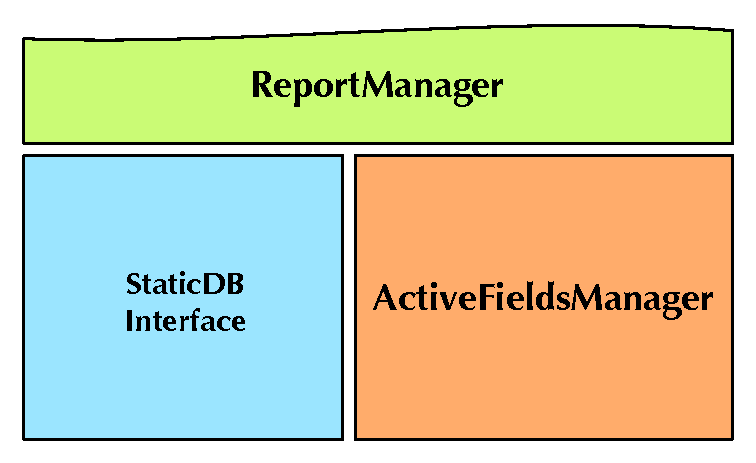
\includegraphics[scale=0.5]{./Images/phases.pdf}
   \caption{Modules of the Dynamic Monitor}
  \label{modules}
  \end{center}
 \end{figure}

\newpage
\subsection{Static analysis results management} 

\paragraph{}
The StaticDB Interface module performs the first step in the computation of the dynamic coverage, that is, the import of the results of the static analysis performed by \datec. In order to maintain an high degree of flexibility, I wanted to represents definitions, uses and associations between pairs as objects that could allow easy and clear comparison and retrieval. 

\paragraph{}
This was the main challenge in the implementation of this component, because the format in which the data is saved into \datec's database is less refined than what I needed to create object from it right away.
More specifically, \datec\ stores the results of the analysis in a MySQL database, in three tables: one for variable definitions, one for uses, and one for the associations defining the pairs. For each field, the 
name, the class, and the \textit{context} (i.e., the chain of methods that leads to a definition/use)  are stored as raw strings:

\begin{table}[H] 
  \centering
    \begin{tabular}{l|l}
    \textbf{completeName} & \textbf{defContext} \\ \hline
    \texttt{<inits.Foo: int i>}  &  \texttt{<inits.SubFoo: void <init>(int)>[8]<inits.Foo: void <init>()>[9]}        
    \end{tabular}
    \caption{An example row of the definitions table}
    \label{table:a_def}
\end{table}

\paragraph{}
The example of Table \ref{table:a_def} illustrates the definition of field \texttt{i} 
of type \texttt{int} belonging to class \texttt{inits.Foo}. This field has been 
assigned a value through means of the constructor of class 
\texttt{inits.SubFoo}, which, at line 8, calls the constructor of class 
\texttt{inits.Foo}. The actual definition occurs at line 9 of this constructor. 

\paragraph{}
As this format is not ideal for manipulation in a complex OO program, I needed to complement the import of data with additional parsing functionalities. This choice was enforced by the fact that \datec\ uses canonical method signatures, while the tool I exploited to perform dynamic instrumentation (see Section \ref{disl})  provides the informations about traced methods in the compact JVM format\footnote{\url{http://docs.oracle.com/javase/1.5.0/docs/guide/jni/spec/types.html\#wp276}}. In light of these limitations, the most convenient course of action was to parse data imported to the database, and transform it accordingly.

\begin{center}
\begin{jcode}[caption={Examples of transformation from canonical to compact form.}]
inits.SubFoo: void <init>(int) => inits/SubFoo: <init>(I)V
inits.Foo: boolean bar(String[],int) => inits/Foo: bar([Ljava/lang/String;I)Z
\end{jcode} 
\end{center}

\paragraph{}
In order to do so I implemented two interfaces, \texttt{FieldParser} and \texttt{MethodParser}. The database interface passes to \texttt{FieldParser} one row at a time; the parser creates a \texttt{Field} object out of it, and delegates to \texttt{MethodParser} the manipulation of the field's context. \texttt{MethodParser} uses a combination of regular expressions and the Guava Libraries\footnote{\url{https://code.google.com/p/guava-libraries/}} to manipulate the context raw string and transform it in a list of \texttt{Method} objects, in order to guarantee good performance. As I import the data, I also create create a \texttt{ContextGraph}. The \texttt{ContextGraph} is a \textit{multigraph} (i.e., a graph in which more than one edge between two nodes is allowed) where each node represents a method of the analyzed program in which at least one definition or one use takes place; it is implemented as a multigraph because there could be multiple call relationships between two methods. The nodes contain all the definitions/uses that occur in that method, and they are connected by directed, valued edges that contain the line number at which the destination method is called. This will be useful at the time of identification of the active fields.

\begin{figure}[H]
  \begin{center}
   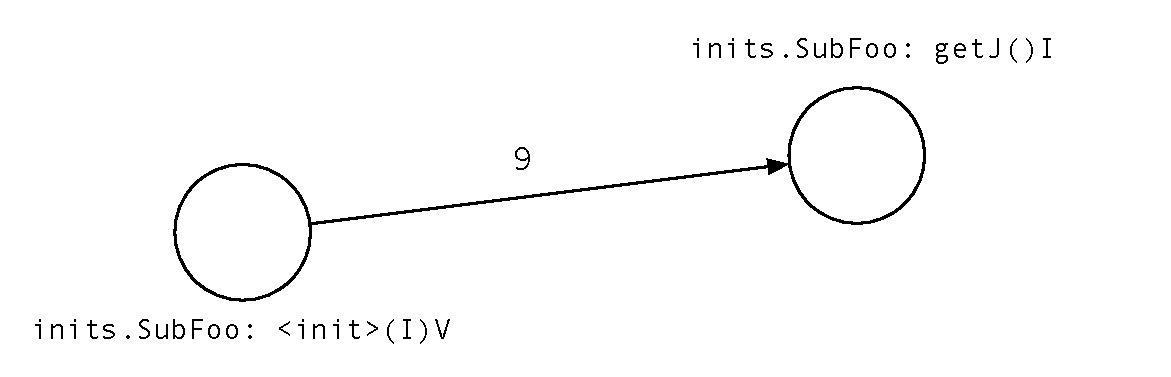
\includegraphics[scale=0.5]{./Images/graphexample.pdf}
   \caption{Example: the constructor of class \texttt{SubFoo} calls method \texttt{getJ} at line 9.}
  \label{gex}
  \end{center}
 \end{figure}

\paragraph{}
This implementation also accounts for the fact that the Static Analysis component is still a work in progress, and, as such, the format of the database may change: the aforementioned interfaces are implemented in two classes, \texttt{DatecFieldParser} and \texttt{DatecMethodParser}, which can parse the current version of the database output. Nevertheless, if a different version was needed, it would be enough to write new classes implementing the interested interfaces and specify their name in the tool's properties. The tool will then take care of exploiting the specified implementation through reflection.

\paragraph{}
For this part, the last concern was performance, because connecting to a database to retrieve the data and then parse it are resource intensive and time consuming operations, even when done efficiently. Moreover, there could be cases in which a user could perform more than one test on the same Java program. In this case, performing again the static analysis and manipulation would be a useless waste.
I addressed this concern by implementing an \texttt{Extractor} class: the class delegates to the database interface the import and manipulation of the data, and then serializes the produced collections. In case that the data in the database is not updated, \texttt{Extractor} avoids estabilishing a connection to the database, and just deserializes the existing data, resulting in increased efficiency.

\subsection{Dynamic instrumentation and coverage}
 
 The Active Fields Manager module implements the logic for the main task of the component, the computation of the data flow coverage achieved by a given test suite. To achieve the task, this module carries out several computations. 
First of all, the module must be able to instrument the program under test in the critical points to trace not only definitions and uses of fields, but also the chain of methods that define their context. 
Secondly, the module has to identify at runtime which definitions and which uses are active and which are killed, so that covered pairs can be properly identified. After the identification of all covered pairs, the third module will take care of generating a report.

\subsubsection{Dynamic instrumentation}\label{disl}
In order to instrument the program in the interested points, I defined four events: definition of a field, use of a field, basic block entry and basic block exit. These events are implemented in four methods of class \texttt{Recorder}:

\begin{itemize}
  \item \texttt{public void onBasicBlockIn(...)} is called upon entry in a basic block;
  \item \texttt{public void onBasicBlockOut(...)} is called upon exit from a basic block;
  \item \texttt{public void onInstanceFieldPut(...)} is called upon definition of a instance field;
  \item \texttt{public void onInstanceFieldGet(...)} is called upon use of a instance field.
\end{itemize}

\paragraph{}
These events acts as a layer on top of the tool I decided to use to capture information at runtime. This choice played a big role, as the component that collects runtime information is the critical part of the coverage computation tool in terms of 
performance; thus, it had to be performed carefully. I was presented with three 
popular solutions to trace the execution of a program in Java:
\begin{enumerate}
  \item Use low level instrumentation libraries (e.g. ASM);
  \item Use Aspect Oriented Programming libraries;
  \item Exploit the Java Debug Interface (JDI);
\end{enumerate}

\paragraph{}
The first solution offers the best performance, but at the same time is the most 
complex to use. The alternative solutions are simpler to use, but their performance are not as good as with ASM. 
Apart from the aforementioned approaches, recently researchers at USI proposed another technique for collecting runtime information of a program called \disl~\cite{Marek}.
 
\paragraph{}\label{eventhandler}
 \disl\ is a framework for dynamic analysis that acts as a middleware between ASM and the user, allowing the definition of 
 simple instrumentation rules through Java annotations, while also promising 
 performance levels higher than those offered by aspect oriented programming and JDI. \disl\ offers
 several predefined templates for instrumentations that I exploited for the analysis. 

\paragraph{}
More specifically, the annotation describes the point in which \disl\ performs code injection. Several parameters can be passed to the annotation, in order to define context information for the instrumentation. I illustrate how \disl\ works using the example reported in Listing~\ref{disl_snippet} that instrument all field definitions. This annotation injects code after (\texttt{@AfterReturning}) the bytecode region specified by the \texttt{BytecodeMarker} \textit{marker}, which in this case captures the allocation of new objects. The annotation \texttt{PutGuard} allowed me to define special \textit{guard} rules to filter out from the instrumentation objects I'm not interested in. Similarly, I specify a \textit{scope} useful to restrict the instrumentation to specific packages. Finally, \disl\ provides informations about the context of the instrumented code region through several parameters: I exploit \texttt{LineNumberStaticContext}, \texttt{FieldStaticContext} (providing \texttt{fieldName(), isArray(), isPrimitive()\dots}),  \texttt{MethodStaticContext} (providing \texttt{thisMethodName(), isPublic()\dots}) and \texttt{DynamicContext} to access context informations and use them to match the information with the one computed by the static analysis. 
  
 \begin{center}
 \begin{minipage}{0.8\textwidth}
    \begin{jcode}[caption={Instrumentation of definitions with DiSL}, label={disl_snippet}]
    @AfterReturning(marker = BytecodeMarker.class, args = "putfield", 
    guard = PutGuard.class, scope = Properties.SCOPE, order = 100)
    public static void afterRetPutField(LineNumberStaticContext lnsc, 
    FieldStaticContext fsc, MethodStaticContext msc, DynamicContext dc)
    { 
        EventHandler.instanceOf().onInstanceFieldPut(...);
    }
    \end{jcode} 
 \end{minipage}
\end{center}

\paragraph{}
Each \disl\ event corresponds to a call to different methods of the \texttt{EventHandler} interface. This interface acts as a communication layer between \disl\ annotations and the four events I defined in the class \texttt{Recorder}. In this way, the tool remains independent from the dynamic instrumentation technology chosen. 

\subsubsection{Coverage}

\paragraph{}
To compute data flow coverage at runtime, the tool must be able to trace which definitions are active or get killed during the execution, and match active definitions with executed uses. This means that, when a definition or a use occurs, the interested field has to be considered active, and the context in which the event occurred has to be registered. As the definition could be subsequently killed before its usage, in order for the coverage to be computed correctly, only the last definition must be marked as active. (Listing \ref{def},\ref{kill}) 

\begin{minipage}{0.5\textwidth}
\begin{jcode}[caption={Variable median is defined (line 5).},label={def}]       
public class MathOps {
  private float median;
  
  public MathOps(){
    median = 0;
  }
  
  ...
}    
\end{jcode} 
\end{minipage}
\begin{minipage}{0.5\textwidth}
\begin{jcode}[caption={Variable median is redefined (line 6): this definition kills the previous one.},label={kill}]       
public class MathOps {

  ...
  
  public void getMedian(...){
    median = computeMedian(...);
    return median;
  }
}  
\end{jcode} 
\end{minipage}

\paragraph{}
In order to easily identify active definitions and uses, the implementation exploits the \texttt{ContextGraph} built at import time. 
When I enter (or exit from) a basic block, I move accordingly in the graph, checking that the line number corresponds to the value of the edge and the destination node signature is the same as the destination basic block instrumented. On the other hand, when a definition or a use occurs, I match it against the static definition and uses present in that node, exploiting two informations: the field's name and the context. The context, that is the chain of methods which led to the definition or use, is obtained by tracking the traversed path inside the graph with a stack of the nodes: whenever I enter a method I push it in the stack, and whenever I exit from it I pop it. These two informations are enough to univocally identify the field. 

 \paragraph{}
 The following step consists in marking the definition/use as active. In order to do so, I needed to track not only informations about the field and its context, but also identify the object that produced it. Otherwise, I could incorrectly cover some pairs that where not actually executed. In addition, I needed some data structure that could allow me to write and retrieve active fields with little overhead. I achieved these objectives by implementing the main interface of this module, \texttt{ActiveFieldsManager}, which manages the registration of active definitions and uses in two \texttt{ActiveFieldMap}s. An \texttt{ActiveFieldMap} is like a Java \texttt{Map}, except from the fact that it supports not only 1-to-1 relationships, but also 1-to-many. This is due to the fact that in the same objects there could be many different definitions and uses.
 
\paragraph{}
When the tool registers a field's definition or use, it records it in the proper \texttt{ActiveFieldMap} with a mapping Object~$\rightarrow$~(Field, Context). Objects are uniquely identified by exploiting their \texttt{identityHashCode}\footnote{\url{http://docs.oracle.com/javase/7/docs/api/java/lang/System.html\#identityHashCode(java.lang.Object)}}. This implementation allows me to quickly register fields as active under one object's \texttt{identityHashCode}, and also kill them by overwriting them.

\paragraph{}
Furthermore, the tool currently implements two different ways of marking fields as active: the tool can either perform a standard coverage, or alternatively perform a wider coverage by taking into account fields' definitions/uses which are implicitly covered:

\begin{table}[H] 
  \centering
    \begin{tabular}{l|l}
    \textbf{completeName} & \textbf{defContext} \\ \hline
    \texttt{<inits.Foo: int i>}  &  \texttt{<inits.SubFoo: void <init>(int)>[8]<inits.Foo: void <init>()>[9]} \\ 
    \texttt{<inits.Foo: int i>}  &  \texttt{<inits.Foo: void <init>()>[9]}        
    \end{tabular}
    \caption{Two definitions of the same field. The second definition can be implicitly covered.}
    \label{table:implicit}
\end{table}

\paragraph{}
In the example from Table \ref{table:implicit}, the second definition can be implicitly covered in case the first 
definition is covered; this behavior can improve the coverage extension. The two different methods are provided through two subclasses  of \texttt{ActiveFieldMap}: \texttt{SimpleActiveFieldMap} and \texttt{SubsumeActiveFieldMap}. The user can specify the preferred behavior by tweaking the tool's properties, and the appropriate implementation will be chosen at runtime.

\paragraph{}\label{associations}
The last step in the computation of the coverage is the marking of definition-use pairs as covered. A marking occurs after the registration of a use as active, because in that case I can safely assume that there is a corresponding active definition. The class \texttt{Associations} contains all the possible definition-use pairs imported from the static analysis, paired with a boolean that mark the pair as covered or not covered. Whenever I register an active use, I retrieve the corresponding active definition (matching by object's \texttt{identityHashCode} and field name),  and mark it as active by switching the boolean value to true. In addition, \texttt{Associations} keeps track of the amount of total pairs in the collection, and the amount of covered pairs. %Finally, the class supports simple iteration provided by two methods: method \texttt{next()}, which returns a tuple composed of (Field, defContex, useContext), and method \texttt{hasNext()}, which tells if there are more tuples to process in the collection. These two methods are useful in the generation of the final report. %questo perzzo � inutile

\subsection{Report generation and presentation of final results}

\paragraph{}
One of the requirements for the tool was the generation of a final report containing the results of the produced coverage. I wanted the user of the tool to be able to create custom report that could suit his needs easily, and without changing the tool's code. 

\paragraph{}
I met this requirement by implementing an \texttt{OutputManager} interface, which features one method: \texttt{write(Associations~a)}. If a user wanted to generate a report in a format different from what is already provided, it would be enough to create a new class implementing the \texttt{OutputManager} interface; this process should be quite straightforward, as I also provide an easy way to iterate through the pairs (see Section \ref{associations}). 

\paragraph{}
As of today, the tools supports two ways of generating a report: either printed to the standard output (this was mainly useful to me for debugging and testing purposes), or saved in a report in XML format. The user can specify the preferred format by switching the dedicated property in the tool's properties, in form of the complete class name in which the report generation is implemented.

\paragraph{}
As an example, the following listing contains a simple report printed to the standard output, which indicates from what database the static analysis informations were extracted, which classes were used to parse it, and which class was used to generate the report.
 
 \newpage
\lstset{basicstyle=\ttfamily}
\begin{jcode}[caption=Example of the application output]
Application is starting.
Database datecm will be parsed according to these classes:
[FIELDPARSER]: ch.usi.star.datec.coverage.context.DatecFieldParser
[METHODPARSER]: ch.usi.star.datec.coverage.context.DatecMethodParser
Results will be presented according to class: 
[OUTPUTSINK]: ch.usi.star.datec.coverage.utilities.StdOut

Db is up to date, reading defs from serialized FieldMap...
Successfully read from serialized StaticFieldMap
Db is up to date, reading uses from serialized FieldMap...
Successfully read from serialized StaticFieldMap
Db is up to date, reading associations from serialized Map...
Successfully read from serialized associations

Application has finished computing coverage.

Time elapsed: 393 ms.
COVERED PAIRS: (3 out of 5)
[Field] <inits.SubFoo: int j> [D]: [inits.SubFoo: setJ(I)V[12]] [U]: [inits.SubFoo: getJ()I[14]] [COVERED]: true
[Field] <inits.SubFoo: int j> [D]: [inits.SubFoo: <init>(I)V[9]] [U]: [inits.SubFoo: getJ()I[14]] [COVERED]: true
[Field] <inits.Foo: int i> [D]: [inits.Foo: setI(I)V[14]] [U]: [inits.Foo: getI()I[12]] [COVERED]: false
[Field] <inits.Foo: int i> [D]: [inits.SubFoo: <init>(I)V[8], inits.Foo: <init>()V[9]] [U]: [inits.Foo: getI()I[12]] [COVERED]: true
[Field] <inits.Foo: int i> [D]: [inits.Foo: <init>()V[9]] [U]: [inits.Foo: getI()I[12]] [COVERED]: false

Shutdown...
\end{jcode}
